\documentclass[10pt]{article}
\usepackage{tikz}
\usetikzlibrary{shapes.misc}
\usepackage[margin=0cm]{geometry}
\pagestyle{empty}
\tikzstyle{every node}=[cross out, draw, red]

\begin{document}

\vspace*{\fill}
\begin{center}
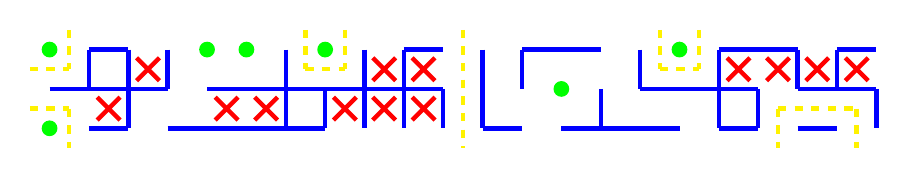
\begin{tikzpicture}[x=0.5cm, y=-0.5cm, ultra thick, blue]
% Walls
    \draw (1,0) -- (2,0);
    \draw (9,0) -- (10,0);
    \draw (12,0) -- (14,0);
    \draw (17,0) -- (19,0);
    \draw (20,0) -- (21,0);
    \draw (0,1) -- (3,1);
    \draw (4,1) -- (10,1);
    \draw (15,1) -- (18,1);
    \draw (19,1) -- (21,1);
    \draw (1,2) -- (2,2);
    \draw (3,2) -- (7,2);
    \draw (11,2) -- (12,2);
    \draw (13,2) -- (16,2);
    \draw (17,2) -- (18,2);
    \draw (19,2) -- (20,2);
    \draw (1,0) -- (1,1);
    \draw (2,0) -- (2,2);
    \draw (3,0) -- (3,1);
    \draw (6,0) -- (6,2);
    \draw (7,1) -- (7,2);
    \draw (8,0) -- (8,2);
    \draw (9,0) -- (9,2);
    \draw (10,1) -- (10,2);
    \draw (11,0) -- (11,2);
    \draw (12,0) -- (12,1);
    \draw (14,1) -- (14,2);
    \draw (15,0) -- (15,1);
    \draw (17,0) -- (17,2);
    \draw (18,1) -- (18,2);
    \draw (19,0) -- (19,1);
    \draw (20,0) -- (20,1);
    \draw (21,1) -- (21,2);
% Pillars
    \fill[green] (0,0) circle(0.2);
    \fill[green] (4,0) circle(0.2);
    \fill[green] (5,0) circle(0.2);
    \fill[green] (7,0) circle(0.2);
    \fill[green] (16,0) circle(0.2);
    \fill[green] (13,1) circle(0.2);
    \fill[green] (0,2) circle(0.2);
% Inner points in accessible cul-de-sacs
    \node at (2.5,0.5) {};
    \node at (8.5,0.5) {};
    \node at (9.5,0.5) {};
    \node at (17.5,0.5) {};
    \node at (18.5,0.5) {};
    \node at (19.5,0.5) {};
    \node at (20.5,0.5) {};
    \node at (1.5,1.5) {};
    \node at (4.5,1.5) {};
    \node at (5.5,1.5) {};
    \node at (7.5,1.5) {};
    \node at (8.5,1.5) {};
    \node at (9.5,1.5) {};
% Entry-exit paths without intersections
    \draw[dashed, yellow] (-0.5,0.5) -- (0.5,0.5);
    \draw[dashed, yellow] (6.5,0.5) -- (7.5,0.5);
    \draw[dashed, yellow] (15.5,0.5) -- (16.5,0.5);
    \draw[dashed, yellow] (-0.5,1.5) -- (0.5,1.5);
    \draw[dashed, yellow] (18.5,1.5) -- (20.5,1.5);
    \draw[dashed, yellow] (0.5,-0.5) -- (0.5,0.5);
    \draw[dashed, yellow] (0.5,1.5) -- (0.5,2.5);
    \draw[dashed, yellow] (6.5,-0.5) -- (6.5,0.5);
    \draw[dashed, yellow] (7.5,-0.5) -- (7.5,0.5);
    \draw[dashed, yellow] (10.5,-0.5) -- (10.5,2.5);
    \draw[dashed, yellow] (15.5,-0.5) -- (15.5,0.5);
    \draw[dashed, yellow] (16.5,-0.5) -- (16.5,0.5);
    \draw[dashed, yellow] (18.5,1.5) -- (18.5,2.5);
    \draw[dashed, yellow] (20.5,1.5) -- (20.5,2.5);
\end{tikzpicture}
\end{center}
\vspace*{\fill}

\end{document}
